\chapter{Requirements Engineering}

\section{Einleitung}
Im folgenden Abschnitt soll die Requirements-Analyse anhand von Use Cases durchgef\"uhrt werden. Requirements Engineering ist ein iterativer Prozess, als Basis f\"ur die Aufwandsch\"atzung wird im Projektplan der erste Schritt durchgef\"uhrt.


\section{Use Case}
\begin{figure}[h]
	\centering
	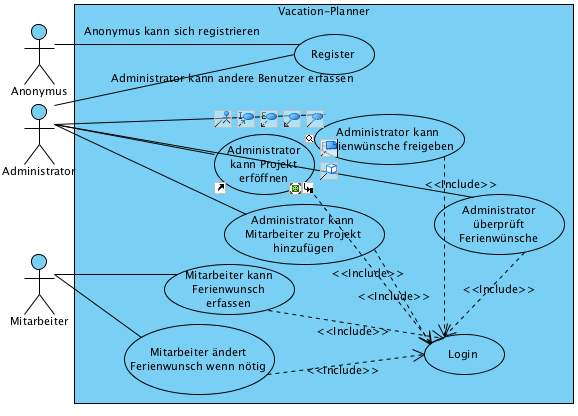
\includegraphics[height=10cm]{orgchart/reqeng_usecase}
	\caption[Use Case Diagramm]{Use Case Diagramm}
\end{figure}

\subsection{Administrator}
Administrator ist die Rolle, welche Mitarbeiter erfasst und f\"ur diese die Ferienw\"unsche beantwortet. Normalerweise handelt es sich bei Administratoren um Team-, Abteilungs- oder Projektleiter. Sie haben bei der Einteilung von Ferien die volle Entscheidungskompetenz. Folgende Use Cases sind f\"ur sie vorgesehen:

\subsubsection{Projekt er\"offnen}
Nach dem Login erfasst der Administrator (Project Manager, Teamleiter, usw.) f\"ur sein Team ein Projekt. Grunds\"atzlich geh\"ort ein Projekt mehreren Administratoren, in einem 2. Projekt wird die zus\"atzliche M\"oglichkeit implementiert, anderen Benutzer Administrator-Rechte f\"urs eigene Projekt zu geben.

\subsubsection{Mitarbeiter in Projekt erfassen}
Projekte alleine sind leere ''Beh\"alter'' f\"ur Mitarbeiter. Um Mitarbeiter ins eigene Projekt zu nehmen, sucht der Administrator nach einem bestehenden User. Sofern es den gesuchten Benutzer im System noch nicht gibt, wird er durch den Administrator neu erfasst. Der neu erfasste Benutzer wird mittels Mail auf diese Aktion aufmerksam gemacht.

\subsubsection{Ferienw\"unsche bearbeiten}
Die vom Mitarbeiter erfassten Ferien k\"onnen durch den Administrator bez\"uglich Status und Termin ver\"andert werden. Die Bewilligung von Ferien wird mittels des Status confirmed / best\"atigt erteilt. Ansonsten gibt es folgende M\"oglichkeiten:
\begin{itemize}
\item erw\"unscht - requested
\item abgelehnt - rejected
\item best\"atigt - confirmed
\end{itemize}


\subsection{Mitarbeiter}
\subsubsection{Ferienwunsch erfassen}
Der Mitarbeiter kann seine Ferienw\"unsche pro Projekt erfassen. Diese befinden sich zu Beginn im Status ''requested'' und k\"onnen vom Administrator in die Status ''rejected'' und ''confirmed'' ge\"andert werden.

\subsubsection{Ferienwunsch bearbeiten}
Sollte ein Ferienwunsch abgelehnt werden, kann er erneut bearbeitet werden, was eine erneute Anfrage beim Administrator zur Folge hat.

\subsection{Mail Versand}
Verschiedene Aktionen und Status-\"Anderungen haben einen Mail-Versand zur Folge:
\subsubsection{Mitarbeiter erfassen}
Wird ein Mitarbeiter  erfasst - egal ob selbst\"andig oder durch einen Administrator - wird ein Mail versendet, in welchem die Erstellung best\"atigt werden muss. Erst dadurch gelangt der User / Mitarbeiter vom Status ''inaktiv'' in den Status ''aktiv''.

\subsubsection{Mitarbeiter hinzuf\"ugen}
Wird ein Mitarbeiter einem Projekt hinzugef\"ugt, wird eine Notifikation an den Mitarbeiter versendet.

\subsubsection{Ferien erfassen}
Werden durch den Mitarbeiter Ferien erfasst, erh\"alt der Administrator ein Mail, bei welchem er auf diese Aktion aufmerksam gemacht wird. Er hat somit die M\"oglichkeit, die W\"unsche schnellstm\"oglich zu best\"atigen.

\subsubsection{Status\"anderung Ferien}
Wird eine Status\"anderung durch den Administrator gemacht, wird ebenfalls ein Mail versendet.
